\chapter{REVISÃO SISTEMÁTICA DA LITERATURA}
\label{cap:revisao}

Este capítulo apresenta os resultados da revisão sistemática desenvolvida no trabalho. O processo identificou 11.904 registros nas quatro fontes consultadas e incluiu 16 estudos na síntese narrativa. A pontuação usada na elegibilidade representou aderência temática ao problema de pesquisa; ela não foi interpretada como medida de qualidade científica.

Esta versão resulta de uma reexecução e auditoria do pipeline, e não de uma simples troca numérica. A execução histórica registrava 17 estudos incluídos; a nova rodada identificou 23 candidatos no limiar operacional e excluiu 7 falsos positivos após a revisão de pertinência, chegando aos 16 estudos atuais. Esses sete registros já estão contabilizados entre os 2.475 excluídos na elegibilidade; não constituem uma exclusão adicional ao fluxo PRISMA. A mudança também está associada ao snapshot atualizado da base e à correção da lógica de scoring, cuja rastreabilidade deve ser lida junto dos estados persistidos e dos artefatos derivados.

\section{Fluxo de Seleção}

A Figura~\ref{fig:prisma-flow} apresenta o fluxo de seleção relatado segundo o PRISMA 2020. Os 11.904 registros do banco consolidado foram avaliados na triagem; 9.413 foram excluídos e 2.491 avançaram para a elegibilidade. Nessa etapa, 2.475 foram excluídos, resultando em 16 estudos incluídos.

\begin{figure}[H]
\centering
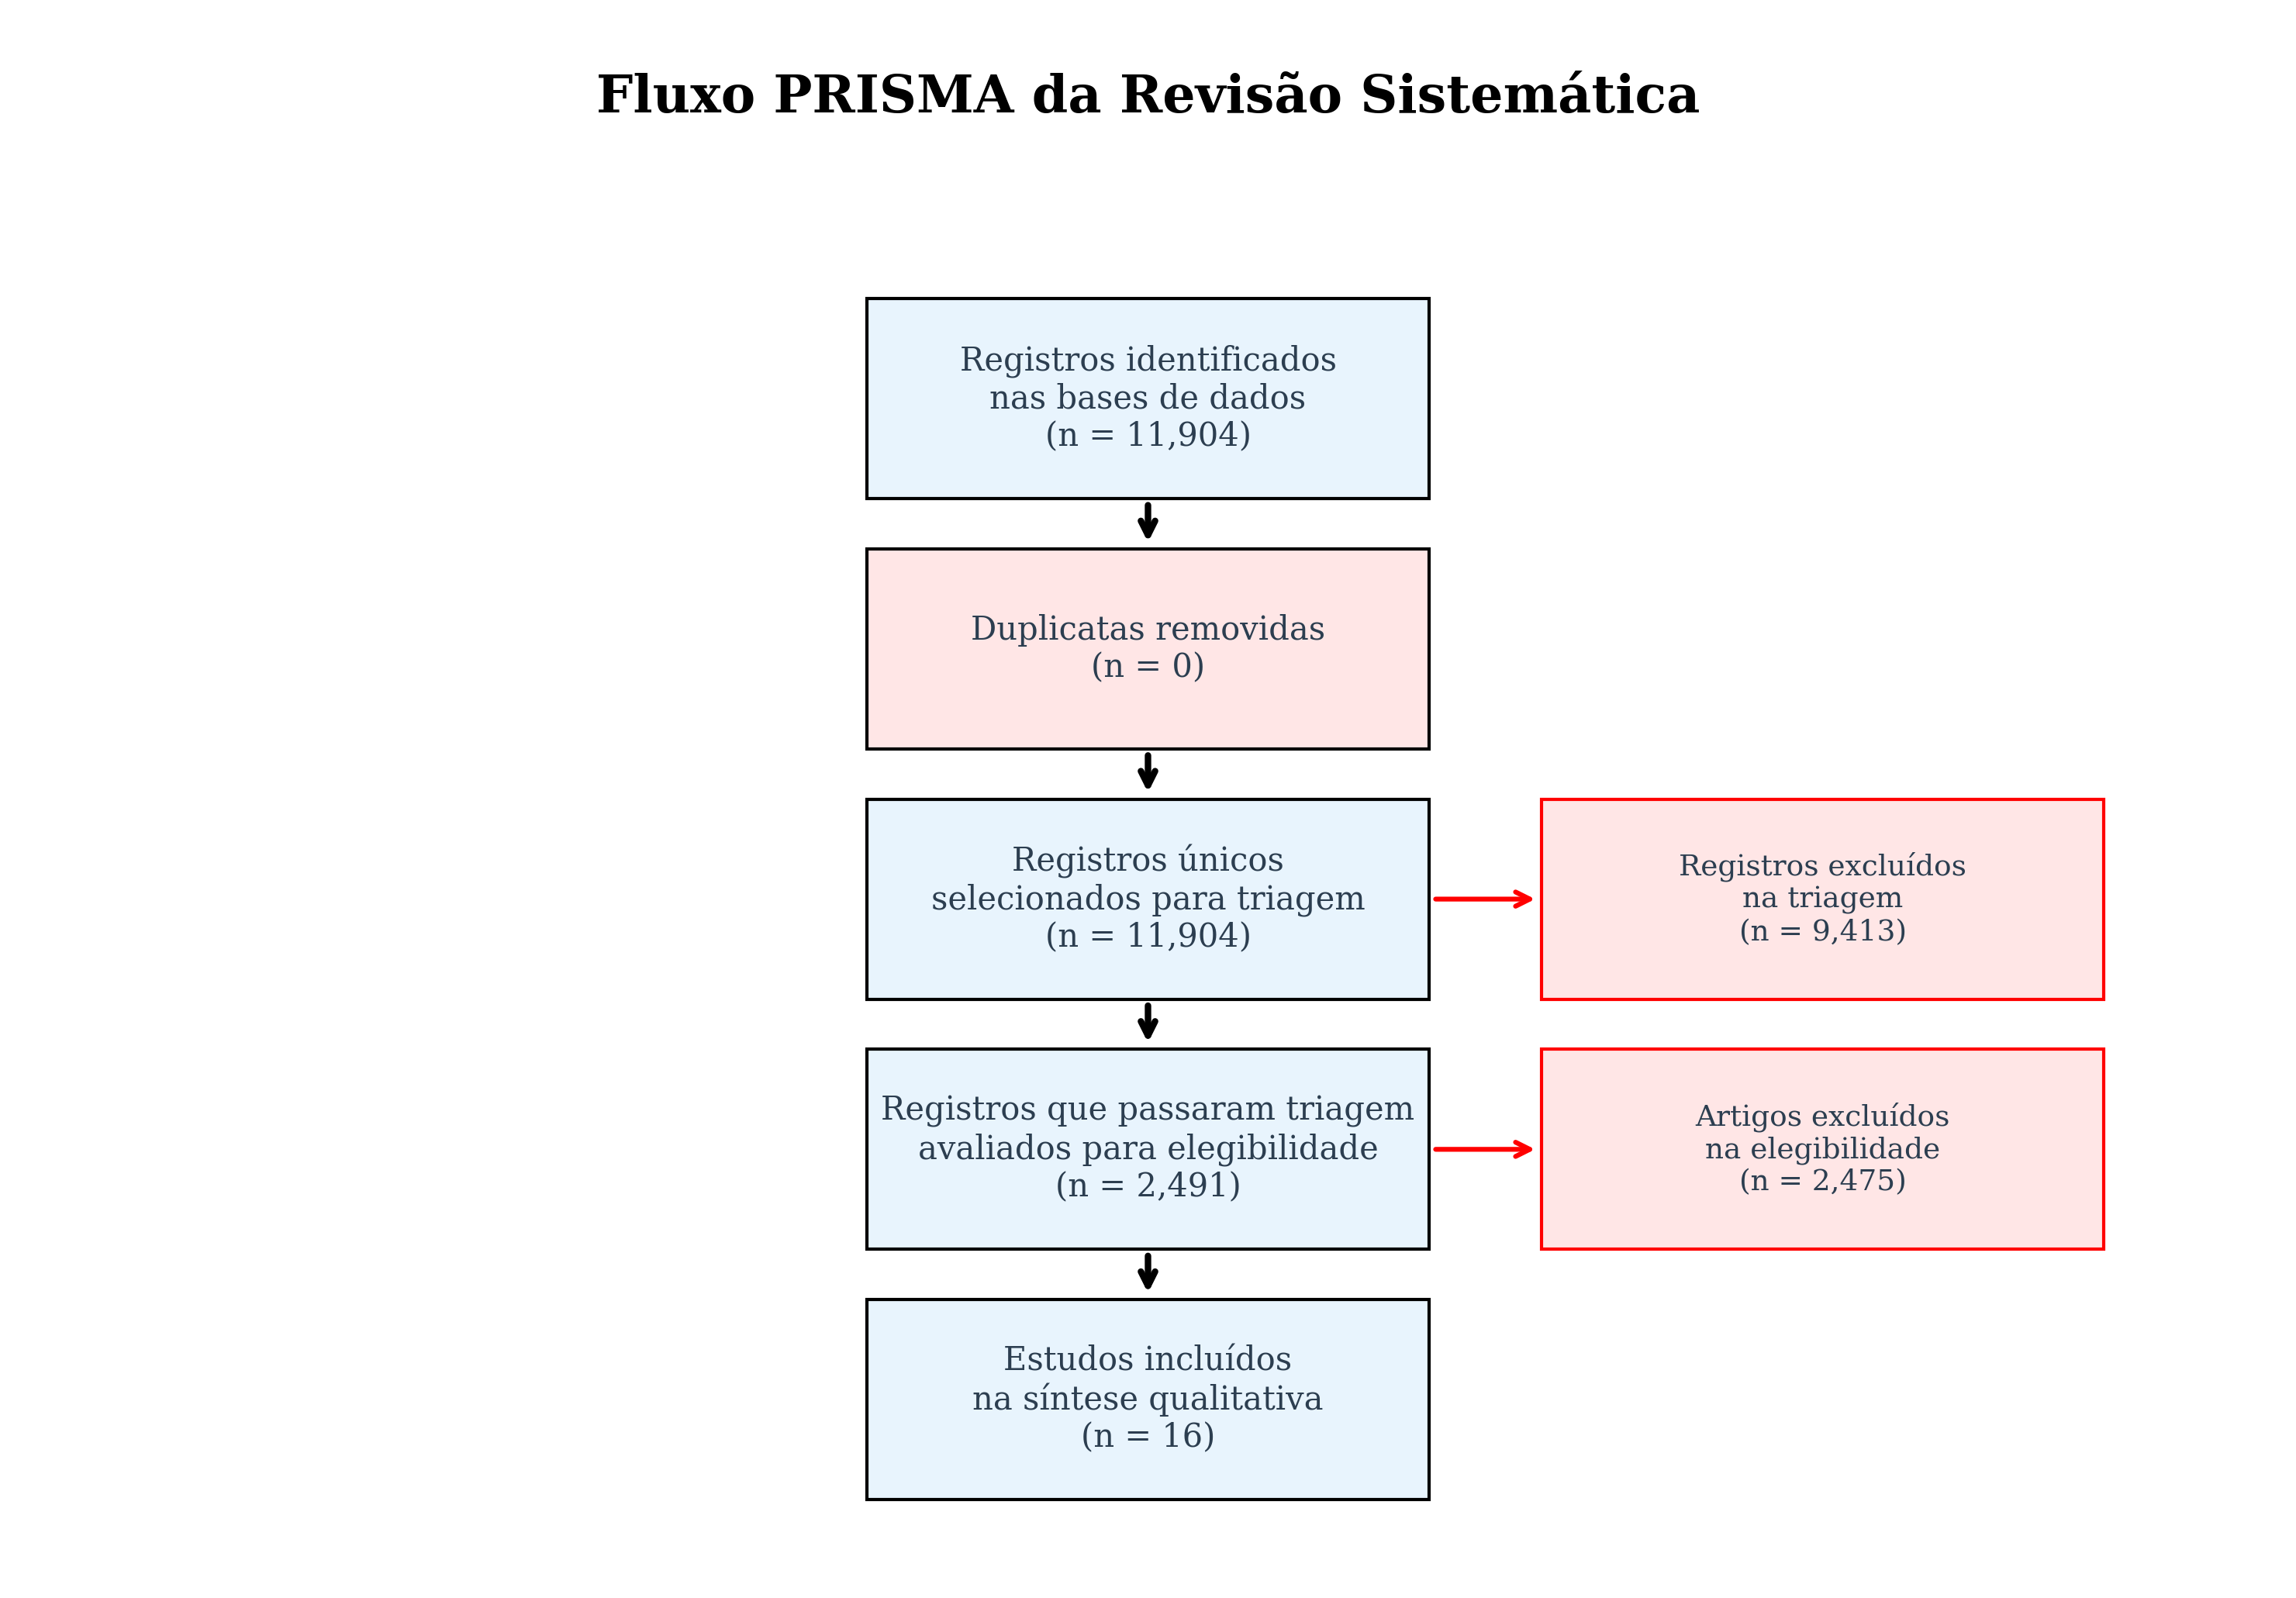
\includegraphics[width=0.85\textwidth]{images/prisma_flow.png}
\caption{Fluxo de seleção da revisão sistemática.}
\label{fig:prisma-flow}
\fonte{Elaborado pelo autor (2026).}
\end{figure}

A Figura~\ref{fig:selection-funnel} representa a redução do conjunto de registros ao longo das etapas.

\begin{figure}[H]
\centering
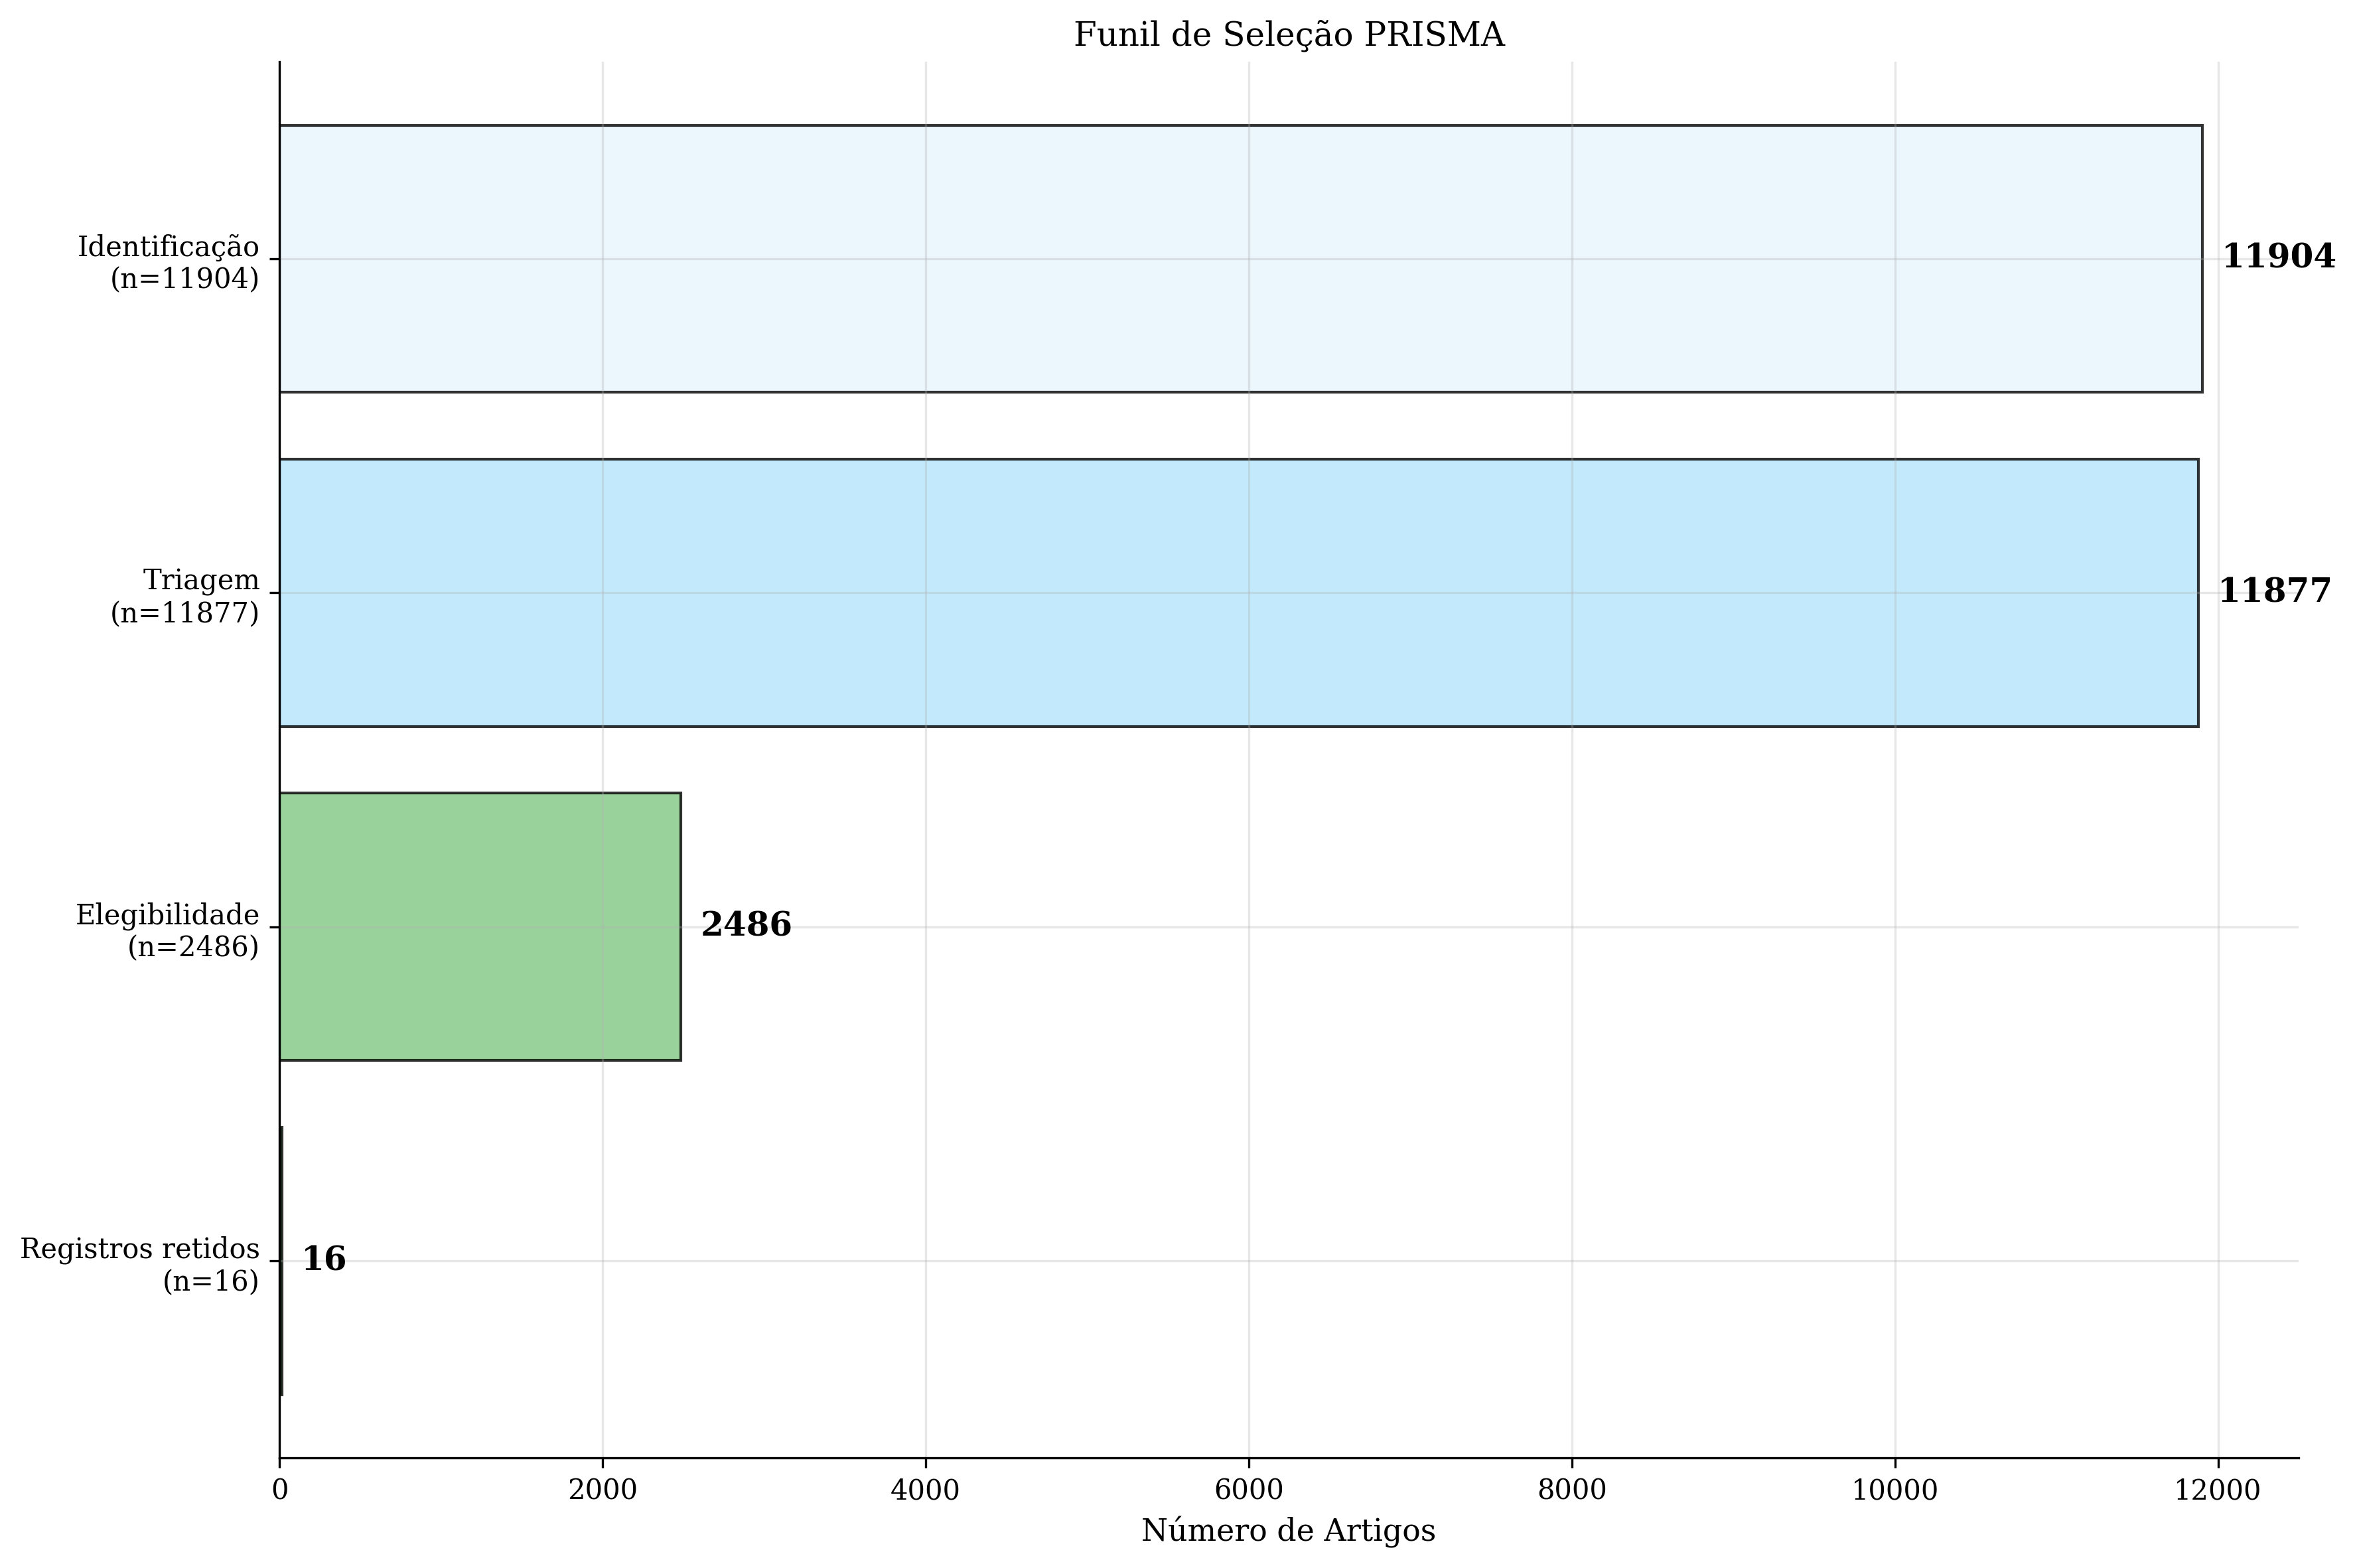
\includegraphics[width=0.85\textwidth]{images/selection_funnel.png}
\caption{Funil de seleção dos estudos.}
\label{fig:selection-funnel}
\fonte{Elaborado pelo autor (2026).}
\end{figure}

\section{Estatísticas Descritivas}

A Tabela~\ref{tab:stats-descritivas} reúne os principais números da revisão. A auditoria de DOI evidencia sobreposição entre registros, embora a flag operacional \texttt{is\_duplicate} não registre remoções neste snapshot. Portanto, ``duplicatas removidas'' igual a zero significa que não houve remoção baseada nessa flag, e não que todos os registros sejam únicos por DOI. A combinação de DOI repetido e similaridade de títulos continua sendo uma decisão de integridade a documentar; a pequena proporção de estudos incluídos decorreu do escopo específico, do filtro de relevância e da auditoria dos candidatos.

A taxa de acertos do \textit{cache} não foi apresentada como métrica fixa. Um acerto ocorreu quando uma consulta foi atendida com uma resposta previamente armazenada, sem nova requisição à API. O contador de acertos é acumulado por entrada do cache, enquanto os eventos são registrados na auditoria; como essa proporção depende do histórico e da expiração das entradas, ela não representa quantidade de registros, qualidade ou evidência de inclusão.

\begin{table}[H]
\centering
\caption{Estatísticas descritivas da revisão sistemática.}
\label{tab:stats-descritivas}
\begin{tabular}{lc}
\hline
\textbf{Métrica} & \textbf{Valor} \\
\hline
Registros identificados & 11.904 \\
Duplicatas removidas na consolidação & 0 (0\%) \\
Registros no banco consolidado & 11.904 \\
Registros avaliados na triagem & 11.904 \\
Registros excluídos na triagem & 9.413 \\
Registros avaliados na elegibilidade & 2.491 \\
Registros excluídos na elegibilidade & 2.475 \\
Estudos incluídos & 16 \\
DOIs normalizados distintos & 10.658 \\
Registros sem DOI & 1.222 \\
Bases consultadas & 4 \\
Consultas bilíngues & 72 (48 EN + 24 PT) \\
Período de cobertura & 2015--2026 \\
\hline
\end{tabular}
\fonte{Elaborado pelo autor (2026).}
\end{table}

A distribuição por fonte é apresentada na Figura~\ref{fig:database-coverage}. A contribuição de cada base foi complementar. Os totais brutos podem conter DOI repetido identificado na auditoria, mas esses casos não foram convertidos automaticamente em exclusões do conjunto vigente.

\begin{figure}[H]
\centering
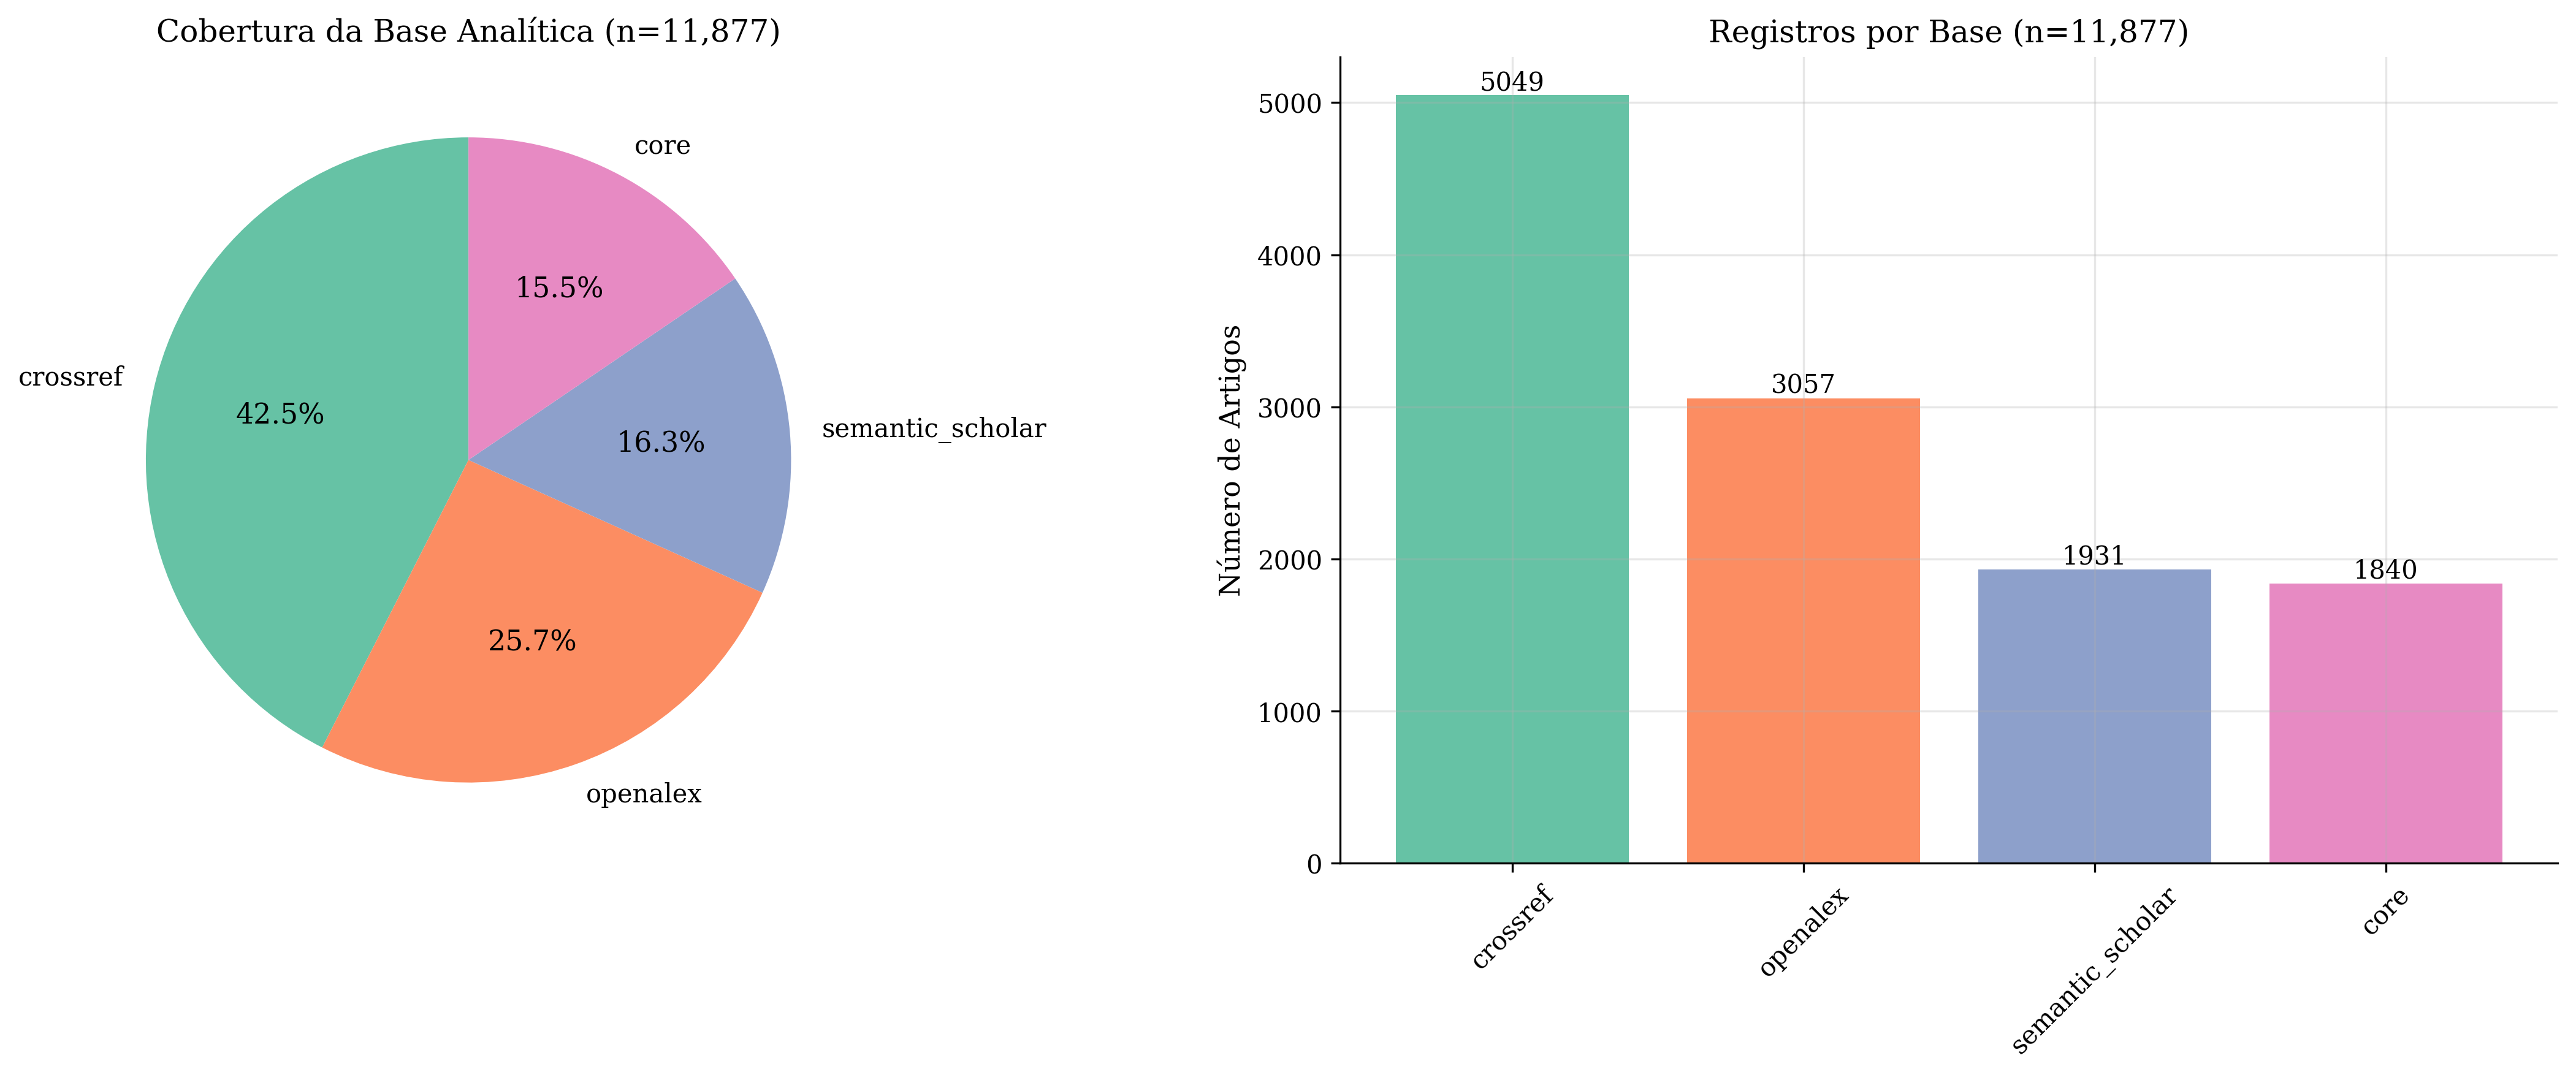
\includegraphics[width=0.85\textwidth]{images/database_coverage.png}
\caption{Registros identificados por fonte científica.}
\label{fig:database-coverage}
\fonte{Elaborado pelo autor (2026).}
\end{figure}

\clearpage
\section{Síntese dos Estudos Incluídos}

Antes da tabela detalhada, três padrões orientam sua leitura. Primeiro, houve predominância de estudos voltados à predição de desempenho ou à classificação de proficiência. Segundo, diferentes algoritmos foram empregados, com recorrência de \textbf{\textit{Random Forest}}, SVM e redes neurais. Terceiro, os resultados não são diretamente comparáveis em todos os casos, pois os estudos utilizaram populações, instrumentos, variáveis e desenhos metodológicos distintos.

Os trabalhos preditivos utilizaram combinações de notas, respostas a itens, características contextuais e registros de interação para estimar categorias ou escores. Outros estudos investigaram personalização, avaliação formativa, recursos pedagógicos ou modelos computacionais de aprendizagem. Essa diversidade ampliou o panorama da revisão, mas também impediu tratar todos os resultados como se medissem o mesmo fenômeno educacional.

Acurácia elevada em uma base específica não demonstra automaticamente que a técnica produzirá o mesmo resultado em outra escola ou população. Da mesma forma, predição de desempenho não equivale a explicar como o estudante aprende matemática. Essas restrições foram incorporadas aos requisitos e aos critérios de avaliação da especificação apresentada no Capítulo~\ref{cap:prototipo}.

Na Tabela~\ref{tab:sintese-estudos-incluidos}, a coluna de resultado preserva o sentido do achado reportado por cada artigo, sem formar um ranking entre estudos. A leitura deve considerar conjuntamente o desenho, a finalidade, a população analisada e as limitações metodológicas relatadas pelos próprios estudos; a reaplicação do MMAT ao conjunto atual permanece pendente. Para registros cuja auditoria bibliográfica ainda exige confirmação em fonte primária, a descrição é provisória e se baseia nos metadados e/ou resumo disponíveis; os números reportados nessas linhas não constituem verificação independente do texto completo.

\begin{landscape}
\fontsize{7.3}{7.8}\selectfont
\setlength{\tabcolsep}{2pt}
\renewcommand{\arraystretch}{0.92}
\begin{longtable}{>{\raggedright\arraybackslash}p{2.6cm}>{\raggedright\arraybackslash}p{3.4cm}>{\raggedright\arraybackslash}p{3.4cm}>{\raggedright\arraybackslash}p{3.1cm}>{\raggedright\arraybackslash}p{2.8cm}>{\raggedright\arraybackslash}p{7.2cm}}
\caption{Síntese dos estudos incluídos.}\label{tab:sintese-estudos-incluidos}\\
\hline
\textbf{Autores/Ano} & \textbf{Tema} & \textbf{Abordagem} & \textbf{Finalidade} & \textbf{Avaliação} & \textbf{Resultado reportado} \\
\hline
\endfirsthead
\multicolumn{6}{c}{\tablename\ \thetable\ -- Continuação}\\
\hline
\textbf{Autores/Ano} & \textbf{Tema} & \textbf{Abordagem} & \textbf{Finalidade} & \textbf{Avaliação} & \textbf{Resultado reportado} \\
\hline
\endhead
\hline
\multicolumn{6}{r}{\textit{Continua na próxima página}}\\
\endfoot
\hline
\endlastfoot
Tjahyadi (2025) \cite{Implementation2025_000} & Predição de desempenho em matemática & EDM; ML; LA & Predição & Desempenho; estatística & Modelo de mineração de dados educacionais para desempenho acadêmico \\
Pejic et al. (2021) \cite{Math2021_001} & Proficiência matemática & ML; avaliação & Predição de proficiência & Desempenho; estatística & Modelo multiclasses para estimar proficiência em avaliação internacional \\
Villegas-Ch et al. (2025) \cite{Villegas2025_6916} & Tutoria inteligente em STEM & ML; tutoria; adaptação; IA & Feedback personalizado & Desempenho; estatística & O registro/resumo informa precisão de 85\% em programação e 78\% em matemática e avaliação positiva do feedback por 80\%; confirmação em fonte primária pendente \\
Sokkhey et al. (2020) \cite{Multimodels2020_002} & Desempenho no ensino médio & ML; LA; predição & Predição & Desempenho; estatística & Comparação de modelos de mineração de dados educacionais \\
Kumar et al. (2022) \cite{Analysis2022_003} & Seleção de atributos & Analítica da aprendizagem & Predição de desempenho & Desempenho & Análise de técnicas de seleção e mineração de dados \\
Özseven e Özseven (2026) \cite{Ozseven2026_6917} & Desempenho em matemática on-line & ML; adaptação; avaliação & Predição & Desempenho & O registro descreve estrutura híbrida com ANFIS, Random Forest e XGBoost para apoiar intervenções personalizadas; confirmação em fonte primária pendente \\
Zhang et al. (2025) \cite{Design2025_004} & Otimização de trajetórias & DL; RL; grafos de conhecimento & Personalização & Retorno de usuários & O registro descreve otimização de trajetórias de aprendizagem personalizada; não deve ser usado como evidência isolada de efetividade \\
Zhang (2023) \cite{Innovative2023_005} & Matemática no ensino superior & IA; adaptação; avaliação & Personalização & Estatística; feedback & O registro descreve modelo de educação curricular incorporando IA; metadados editoriais ainda requerem confirmação \\
Depren et al. (2017) \cite{Identifying2017_006} & Classificação no TIMSS & LA; avaliação & Predição & Estatística; feedback & Comparação de desempenhos de métodos de mineração de dados educacionais \\
Uskov et al. (2019) \cite{Machine2019_007} & Analítica preditiva em STEM & ML; LA; predição & Predição & Desempenho; estatística & Benchmark de algoritmos para predição de desempenho acadêmico \\
MacLellan (2017) \cite{Computational2017_008} & Modelos computacionais de aprendizagem & Tutoria; avaliação; predição & Tutoria e modelagem & Estatística & Modelos computacionais para desenvolvimento de tutores e previsão de comportamento \\
Käser Jacober (2025) \cite{Kaser2025_6918} & Aprendizagem matemática assistida por computador & Tutoria; avaliação; predição & Personalização & Feedback; desempenho; estatística & O registro descreve sistema adaptativo baseado em modelo de habilidades matemáticas e estudos com usuários; confirmação em fonte primária pendente \\
Milićević et al. (2024) \cite{Machine2024_009} & Apoio ao ensino de matemática & ML; LA; predição & Predição e apoio & Desempenho & Métodos de aprendizado de máquina como ferramenta auxiliar ao ensino \\
Echeveria et al. (2025) \cite{Echeveria2025_6920} & Mentalidade matemática & ML; LA; predição & Intervenção precoce & Desempenho & O registro/resumo informa acurácia de 98,8\% para a predição de mentalidades matemáticas; confirmação em fonte primária pendente \\
Imperatrice et al. (2025) \cite{Imperatrice2025_6921} & Ensino inclusivo de matemática & Adaptação; IA; avaliação & Personalização e inclusão & Feedback & O registro descreve proposta de intervenção com IA, visualizações e avaliação pré/pós-teste; identificação bibliográfica e fonte primária requerem confirmação \\
Zeng (2025) \cite{Zeng2025_6923} & Carga cognitiva na resolução de problemas & ML; adaptação; IA & Reconhecimento de estados cognitivos & Estatística & O registro/resumo informa 77,21\% (regressão logística) e 75\% (SVM) para modelos multimodais; confirmação em fonte primária pendente \\
\end{longtable}
\fonte{Elaborado pelo autor (2026).}
\end{landscape}

\section{Avaliação Metodológica com o MMAT}
\label{sec:qualidade-estudos}

O MMAT 2018 foi definido como instrumento de apreciação metodológica conforme o desenho de cada estudo \cite{MMAT2018}. As respostas S (``Sim''), N (``Não'') e ND (``Não é possível determinar'') devem ser mantidas por critério, sem média, ranking ou categoria geral. A atualização do banco alterou o conjunto incluído de 17 para 16 estudos, mas os julgamentos disponíveis no arquivo histórico correspondem à versão anterior e não incluem os seis novos estudos. Por isso, a reaplicação do instrumento ao conjunto atual é uma pendência explícita desta consolidação, e a tabela histórica não é apresentada como resultado final.

A tabela MMAT final deverá ser gerada automaticamente a partir do arquivo versionado \texttt{research/data/\allowbreak{}mmat\_assessments.csv} após a reaplicação aos 16 estudos atuais. Até essa atualização, os critérios apresentados no arquivo histórico não devem ser interpretados como avaliação completa do conjunto vigente.

O arquivo histórico registra, para sua composição anterior, limitações como descrição incompleta dos dados, controle insuficiente de variáveis de confusão e representatividade restrita. Essas observações não são uma avaliação MMAT dos 16 estudos atuais. Após a reaplicação, as limitações deverão ser consideradas na força atribuída a cada evidência, sem ordenar os estudos por uma nota.

\section{Tendências e Lacunas}

A análise dos estudos indicou concentração em modelos preditivos e etiquetas de aprendizado de máquina. Abordagens de explicabilidade, integração curricular, avaliação longitudinal e participação docente apareceram com menor frequência nos metadados disponíveis; essa leitura deverá ser confirmada na reaplicação metodológica aos 16 estudos atuais.

As principais lacunas identificadas foram:

\begin{itemize}
    \item validação limitada em contextos escolares diversos;
    \item pouca discussão sobre como indicadores computacionais se relacionam à aprendizagem matemática;
    \item escassez de análises de equidade e possíveis vieses;
    \item baixa disponibilidade de dados e códigos para reprodução;
    \item pouca integração entre resultados dos modelos e decisões pedagógicas;
    \item ausência de alinhamento explícito com referenciais curriculares brasileiros em grande parte dos estudos.
\end{itemize}

\section{Limitações da Revisão}

A revisão foi realizada por um único pesquisador, com suporte automatizado para deduplicação, triagem e organização dos registros. Não houve dupla revisão independente. A elegibilidade de grande parte dos registros foi avaliada a partir de títulos, resumos e metadados, pois nem todos os textos completos estavam disponíveis.

Embora a revisão por pares e a disponibilidade de texto completo tenham sido definidas como critérios planejados, a auditoria bibliográfica ainda classifica alguns registros atuais como cautela editorial, veículo ausente ou fonte institucional. Assim, o estado ``incluído'' representa o snapshot operacional atual e não confirma, por si só, a validação bibliográfica individual de cada estudo.

O protocolo não foi registrado prospectivamente. Foram adotados princípios de planejamento compatíveis com o PRISMA-P, mas não se afirmou conformidade integral. O PRISMA 2020 foi utilizado para orientar o relato do processo.

As fontes consultadas possuem cobertura predominantemente anglófona, e a busca foi limitada a português e inglês. A heterogeneidade dos desenhos, populações e métricas impediu uma síntese quantitativa conjunta. Além disso, a avaliação MMAT por revisor único está sujeita a divergências interpretativas.

\section{Contribuições para a Especificação do Protótipo}

A revisão forneceu a base empírica para a especificação do protótipo. A recorrência de tarefas preditivas justificou a inclusão de modelos de aprendizado de máquina entre as alternativas de modelagem, enquanto a heterogeneidade das bases impôs critérios explícitos de seleção e validação. As lacunas de explicabilidade, integração curricular, participação docente e reprodutibilidade foram convertidas em requisitos técnicos e pedagógicos.

Dessa forma, os resultados da revisão não foram tratados apenas como levantamento bibliográfico. Eles sustentaram as decisões consolidadas no Capítulo~\ref{cap:prototipo}, preservando a distinção entre evidências reportadas na literatura e resultados produzidos pelo próprio trabalho.

%--------- FIM REVISÃO SISTEMÁTICA ------------
